\documentclass[11pt,a4paper]{scrartcl}

% Pakete
\usepackage[english]{babel}
\usepackage[UKenglish]{isodate}
\usepackage{xcolor}
\usepackage{graphicx}
\usepackage{amsmath}
\usepackage{amssymb}
\usepackage{nicefrac}
\usepackage[utf8]{inputenc}
\usepackage{siunitx}
\sisetup{
output-decimal-marker={.},
exponent-product=\cdot }
\usepackage{esvect}
\usepackage{eqnarray}
\usepackage{placeins}
\usepackage{scrpage2}
\usepackage{nameref}
\usepackage{upgreek}
\usepackage{caption}
\usepackage{subcaption}
\usepackage{bm}
\usepackage{mwe}
\usepackage{tcolorbox}
\usepackage{listings}
\usepackage{xstring}
\usepackage{stringstrings}
\usepackage{floatflt}
\usepackage{pgfplots}
\usepackage{tikz}
%\usepackage{physics}


% Custom colors
\definecolor{deepblue}{rgb}{0,0,0.5}
\definecolor{deepred}{rgb}{0.6,0,0}
\definecolor{deepgreen}{rgb}{0,0.5,0}
\DeclareFixedFont{\ttb}{T1}{txtt}{bx}{n}{12} % for bold
\DeclareFixedFont{\ttm}{T1}{txtt}{m}{n}{12}  % for normal

% tikz
\usetikzlibrary{arrows}

% caption setup
\captionsetup[subfigure]{labelformat=simple, labelsep=colon}
\renewcaptionname{english}{\figurename}{Fig.}
\renewcommand{\thesubfigure}{\arabic{figure}.\arabic{subfigure}}
\renewcommand{\thesubtable}{\arabic{table}.\arabic{subtable}}

% Listning Einstellungen
\lstloadlanguages{python}       % Default highlighting set to "python"
\DeclareCaptionFont{white}{\color{white}}
\DeclareCaptionFormat{listing}{%
  \parbox{0.99\textwidth}{\colorbox{gray}{\parbox{0.99\textwidth}{#1#2#3}}\vskip+5pt}}
\captionsetup[lstlisting]{format=listing, labelfont=white, textfont=white}
\lstset{frame=lrb,xleftmargin=\fboxsep,xrightmargin=-\fboxsep}
\pagestyle{empty}
\lstset{escapeinside={<@}{@>}}
\lstdefinestyle{MyPythonStyle}{
		language=Python,
		numbers=left,
		breaklines=true,
		basicstyle=\ttm,
		otherkeywords={self},             % Add keywords here
		keywordstyle=\ttb\color{deepblue},
		emph={MyClass,__init__},          % Custom highlighting
		emphstyle=\ttb\color{deepred},    % Custom highlighting style
		stringstyle=\color{deepgreen},
		frame=tb,                         % Any extra options here
		showstringspaces=false            % 
		}
\lstdefinestyle{MyCStyle}{
		language=C,
		numbers=left,
		tabsize=4,
		breaklines=true,
		basicstyle=\ttm,
		otherkeywords={self},             % Add keywords here
		keywordstyle=\ttb\color{deepblue},
		emph={MyClass,__init__},          % Custom highlighting
		emphstyle=\ttb\color{deepred},    % Custom highlighting style
		stringstyle=\color{deepgreen},
		frame=tb,                         % Any extra options here
		showstringspaces=false            % 
		}
\renewcommand{\lstlistingname}{Code block}
\renewcommand{\lstlistlistingname}{List of \lstlistingname s}

% Griechische Buchstaben vereinheitlichen
\renewcommand{\alpha}{\upalpha}
\renewcommand{\beta}{\upbeta}
\renewcommand{\gamma}{\upgamma}
\renewcommand{\delta}{\updelta}
\newcommand{\w}{\omega}
\newcommand{\la}{\lambda}

% Eigene mathematische Kommandos
\newcommand{\dd}{\text{d}} 							% Differential
\newcommand{\p}{\partial} 								% Partielles Differential
\newcommand{\D}{\Delta} 								% Fehler / Laplace
\newcommand{\order}[1]{\mathcal{O}\left( #1 \right)}
\newcommand{\abs}[1]{\left| #1\right|} 					% Betrag
\newcommand{\Max}[1]{\max \left\lbrace #1\right\rbrace} % max{}
\newcommand{\Min}[1]{\min \left\lbrace #1\right\rbrace} % min{}
\newcommand{\diff}[2]{\frac{\text{d} #1}{\text{d} #2}}	% Ableitung
\newcommand{\pdiff}[2]{\frac{\partial #1}{\partial #2}} % Partielle Ableitung
\newcommand{\errprop}[2]{\left| \frac{\partial #1}{\partial #2}\right| \cdot \Delta #2}
														% Fehlerfortpflanzung
\newcommand{\rel}[1]{\frac{\Delta #1}{#1}}				% Relativer Fehler

% Eigene trigonometrische Funktionen
\newcommand{\Exp}[1]{\text{exp}\left( #1 \right)}		% exp()
\newcommand{\Ln}[1]{\text{ln}\left( #1 \right)}			% ln()
\newcommand{\Log}[1]{\text{log}\left( #1 \right)}		% log()
\newcommand{\Sin}[1]{\text{sin}\left( #1 \right)}     	% sin()
\newcommand{\Cos}[1]{\text{cos}\left( #1 \right)}		% cos()
\newcommand{\Sinz}[1]{\text{sin}^2\left( #1 \right)}	% sin^2()
\newcommand{\Cosz}[1]{\text{cos}^2\left( #1 \right)}	% cos^2()
\newcommand{\Tan}[1]{\text{tan}\left( #1 \right)}		% tan()
\newcommand{\Asin}[1]{\text{asin}\left( #1 \right)}		% asin()
\newcommand{\Acos}[1]{\text{acos}\left( #1 \right)}		% acos()
\newcommand{\Atan}[1]{\text{atan} \left( #1 \right)}	% atan()

% Eigene Vektor Kommandos
\newcommand{\tovec}[2]{\begin{pmatrix}#1\\ #2\end{pmatrix}}	% 2D-Vektor
\newcommand{\trvec}[3]{\begin{pmatrix}#1\\ #2\\ #3\end{pmatrix}}	% 3D-Vektor	
\newcommand{\ovec}[1]{\boldsymbol{#1}}

% Eigene Referenz-Kommandos
\newcommand{\eref}[1]{(\ref{#1})}						% Gleichungen
\newcommand{\sref}[2]{\subref{#2}}						% Unterabbildungen
\newcommand{\kref}[1]{\ref{#1} \glqq\nameref{#1}\grqq}  % Kapitel
\newcommand{\lref}[1]{$[#1]$}							% Quellen: \newcommand{\lit}{1} => \lref{\lit}

% listing commandos
\newcommand{\listfile}[7][MyPythonStyle]{
\lstinputlisting[linerange={#4-#5}, firstnumber=#4, caption={#6} \hfill script:  #3, label=#7, style=#1]{#2}}
% arguments:
% \listfile[style]{location/filename}{filename}{firstline}{lastline}{title}{label}
% Imports code from a file 
% You will have to escape the filename and the title
% style is an optional argument.

\newcommand{\ls}[1]{\lstinline@#1@}

% using \lstinline@code@ for code in line
% works with every sign instead of @

% commands for this task
\newcommand{\ua}{AU}
\newcommand{\vecx}[1]{\ovec{x}^{(#1)}}
\newcommand{\vecv}[1]{\ovec{v}^{(#1)}}
\newcommand{\veca}[1]{\ovec{a}^{(#1)}}
\newcommand{\vecF}[1]{\ovec{F}^{(#1)}}
\newcommand{\vecr}[1]{\ovec{r}^{(#1)}}
\newcommand{\nx}[1]{x^{(#1)}}
\newcommand{\nv}[1]{v^{(#1)}}
\newcommand{\na}[1]{a^{(#1)}}
\newcommand{\nm}[1]{m^{(#1)}}
\newcommand{\nF}[1]{F^{(#1)}}
\newcommand{\nr}[1]{r^{(#1)}}
\newcommand{\Ekin}{E_\text{kin}}
\newcommand{\Ekino}{E_{\text{kin},0}}
\newcommand{\fr}{f_\text{re}}
\newcommand{\fij}{\ovec{f}_{ij}}
\newcommand{\rij}{\ovec{r}_{ij}}
\newcommand{\fji}{\ovec{f}_{ji}}
\newcommand{\rji}{\ovec{r}_{ji}}
\newcommand{\rj}{\ovec{r}_{j}}
\newcommand{\ri}{\ovec{r}_{i}}



% Kopf-/Fusszeile
\pagestyle{scrheadings}
\clearscrheadfoot
\chead{Simulation Methods in Physics I}
\ihead{Worksheet 3}
\ohead{\today}
\ofoot{\pagemark}
\ifoot{Michael Marquardt, Cameron Stewart}

\begin{document}

% Titelseite
\begin{titlepage}

\ \\ \ \\ \ \\

\center\textbf{
\begin{large}
Simulation Methods in Physics I
\end{large} \\ \ \\
\begin{Large}
Worksheet 3: Molecular Dynamics 2 and Observables
\end{Large}}   \\ \ \\
\ \\ \ \\

\begin{tabular}{lll}
Students: &Michael Marquardt &Cameron Stewart\\ 
matriculation numbers: &3122118 &3216338\\
\end{tabular}

\end{titlepage}

% Inhaltsverzeichnis

% -------------------------------------- Begin Of Document ----------------------------------------

\section{Command line parameters}

For the simulation different command line parameters were defined.
In the following code blocks you can see them.
They will be explained during the report.

\listfile{../src/ljsim.py}{src/ljsim.py}{9}{18}{Commands for ljsim.py}{comsim}

\listfile{../src/ljanalyze.py}{src/ljanalyze.py}{8}{15}{Commands for ljanalyze.py}{comana}

\section{Restart the program where left it}

First we want to change the programm in a way, that it is able to restart the simulation where it ended last time.
The first thing that we have to do is to store the necessary information about the end state of the system, the position x and velocity v of each particle, into the file ljsim.dat. 
This happens in code block \ref{3storing}.
Furthermore there are the new variables Ts and Ps.
The represent the temperature and pressure of the system over time and will be explained in the next chapter.

\listfile{../src/ljsim.py}{src/ljsim.py}{208}{212}{Storing data}{3storing}

%\begin{lstlisting}[
%	style=MyPythonstyle, 
%	caption=Storing data
%	\hfill script:\ \ \ 
%	src/ljsim.py, 
%	label=3storing, 
%	firstnumber=208
%	]
%# write out simulation data
%print("Writing simulation data to {}.".format(datafilename))
%datafile = open(datafilename, 'w')
%pickle.dump([ts, Es, Ts, Ps, x, v], datafile)
%datafile.close()
%\end{lstlisting}

Now this data must be read by ljsim.py.
Therefore we define a command line parameter \ls{--cont} which accepts as argument the time for which the simulation should be continued (code block \ref{comsim}).
If the parameter is not used the simulation will start new.
Furtehrmore there is another argument \ls{--time} which takes the simulationtime for a new simulation.
The code in code block \ref{3cont} does exactly this.

\listfile{../src/ljsim.py}{src/ljsim.py}{65}{82}{Continue simulation}{3cont}


\section{Calculating Temperature and Pressure}

\subsection*{Deviation of the pressure}

The virial of a system is defined as:
\begin{align}
G
	&=\sum_i^N\ovec{p}_i\cdot\ovec{r}_i
	\label{4p1}
\end{align}

In the case
\begin{align}
0
	&=\left\langle\diff{G}{t}\right\rangle 
	=\left\langle\sum_i^N\frac{\ovec{p}_i^2}{m_i}\right\rangle+\sum_i^N\left\langle\ovec{F}_i\cdot\ovec{r}_i\right\rangle
	\label{4p2}
\end{align}

the following equation can be derived:
\begin{align}
-\sum_i^N\left\langle\ovec{F}_i\cdot\ovec{r}_i\right\rangle
	&=2\left\langle\sum_i^N\frac{\ovec{p}_i^2}{2m_i}\right\rangle
	=2\left\langle E_\text{kin}\right\rangle
	=3Nk_BT
	\stackrel{\text{id. gas}}{=}3PV
	\label{4p3}
\end{align}

For an pair interaction (like in the simulation) let the forces $\fij$ and the vectors $\rij$ be defined as follows:
\begin{align}
\rij
	&=\rj - \ri
	\label{4rij}\\
\fij 
	&= f_\text{lj}(\rij^2)\cdot\frac{\rij}{\abs{\rij}}
	\label{4fij}
\end{align}

With this knowldege we can derive the pressure of the system:
\begin{align}
P
	&=P_\text{id. gas} + P_\text{interaction}
	\label{4p4}\\
	&=\frac{Nk_BT}{V} + \frac{1}{3V}\sum_i^N\left\langle\ovec{F}_i\cdot\ovec{r}_i\right\rangle
	\label{4p5}\\
	&=\frac{1}{3V}\left[\left\langle\sum_i^N\frac{\ovec{p}_i^2}{2m_i}\right\rangle + \left\langle\sum_{i,j\neq i}^N-\fij\cdot\ovec{r}_i\right\rangle\right]
	\label{4p6}\\
	&=\frac{1}{3V}\left[\left\langle\sum_i^N\frac{\ovec{p}_i^2}{2m_i}\right\rangle + \left\langle\sum_{i,j>i}^N\fij\cdot\rj-\fij\cdot\ri\right\rangle\right]
	\label{4p7}\\
	&=\frac{1}{3V}\left[\left\langle\sum_i^N\frac{\ovec{p}_i^2}{2m_i}\right\rangle + \left\langle\sum_{i,j>i}^N\fij\cdot\rij\right\rangle\right]
	\label{4p8}\\
	&=\frac{1}{3V}\left[ 2\left\langle E_\text{kin}\right\rangle + \left\langle\sum_{i,j>i}^N\fij\cdot\rij\right\rangle\right]
	\label{4p9}
\end{align}
\section{Molecular Dynamics at a Desired Temperature}

\begin{figure}[ht]

Obs.
\hfill
\begin{subfigure}{0.3\textwidth}
\centering
$T_0 = 0.3$
\end{subfigure}
\hfill
\begin{subfigure}{0.3\textwidth}
\centering
$T_0 = 1.0$
\end{subfigure}
\hfill
\begin{subfigure}{0.3\textwidth}
\centering
$T_0 = 2.0$
\end{subfigure}

T
\hfill
\begin{subfigure}{0.3\textwidth}
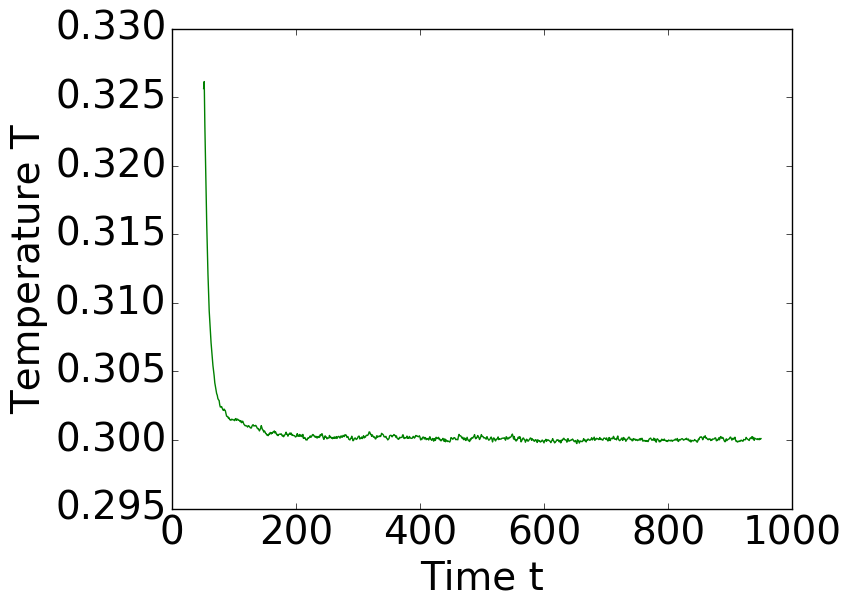
\includegraphics[width=\textwidth]{../dat/avTemperature_T0d3_M100.png}
\end{subfigure}
\hfill
\begin{subfigure}{0.3\textwidth}
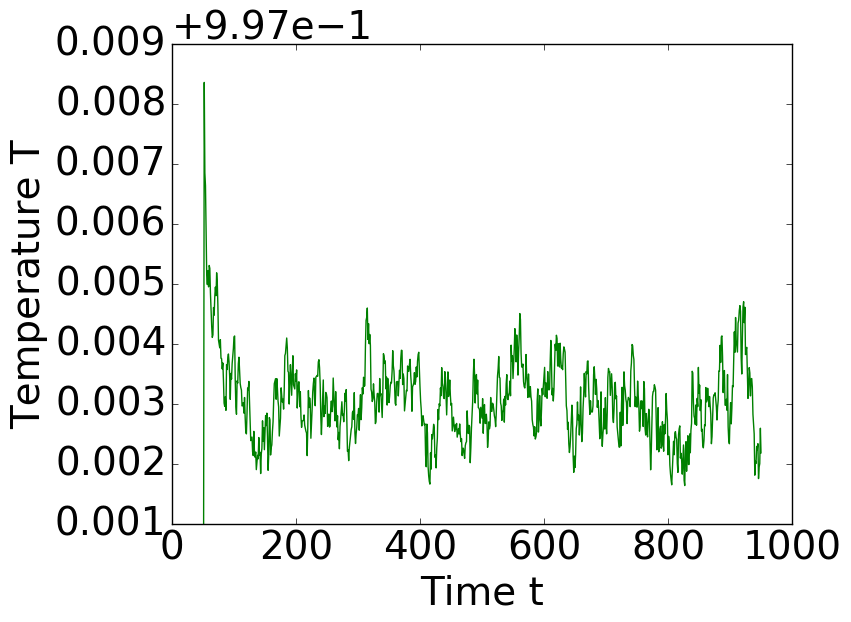
\includegraphics[width=\textwidth]{../dat/avTemperature_T1d0_M100.png}
\end{subfigure}
\hfill
\begin{subfigure}{0.3\textwidth}
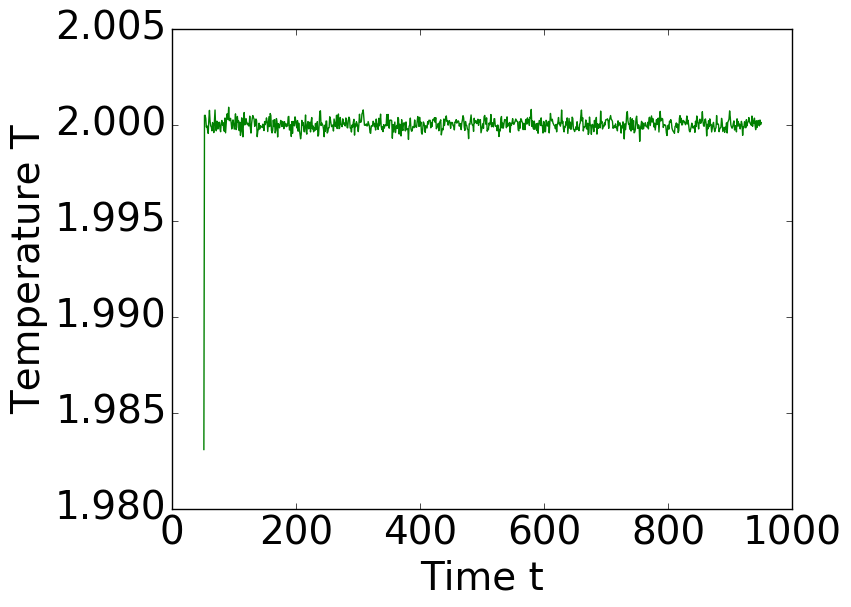
\includegraphics[width=\textwidth]{../dat/avTemperature_T2d0_M100.png}
\end{subfigure}

E
\hfill
\begin{subfigure}{0.3\textwidth}
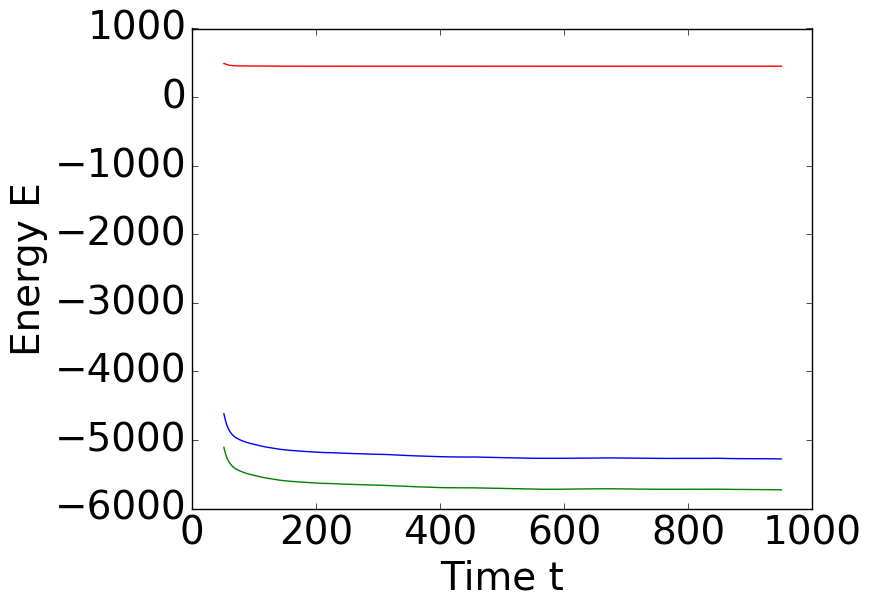
\includegraphics[width=\textwidth]{../dat/avEnergies_T0d3_M100.png}
\end{subfigure}
\hfill
\begin{subfigure}{0.3\textwidth}
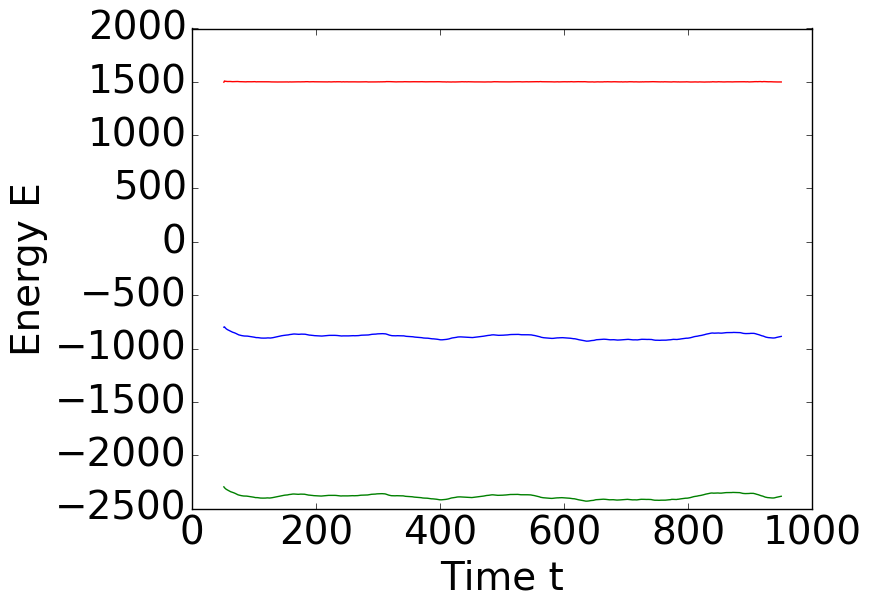
\includegraphics[width=\textwidth]{../dat/avEnergies_T1d0_M100.png}
\end{subfigure}
\hfill
\begin{subfigure}{0.3\textwidth}
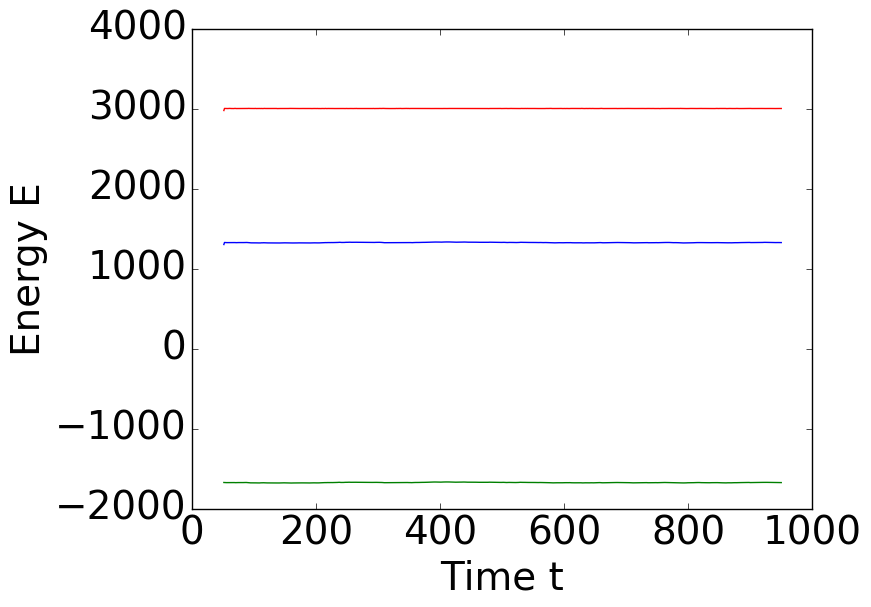
\includegraphics[width=\textwidth]{../dat/avEnergies_T2d0_M100.png}
\end{subfigure}

U
\hfill
\begin{subfigure}{0.3\textwidth}
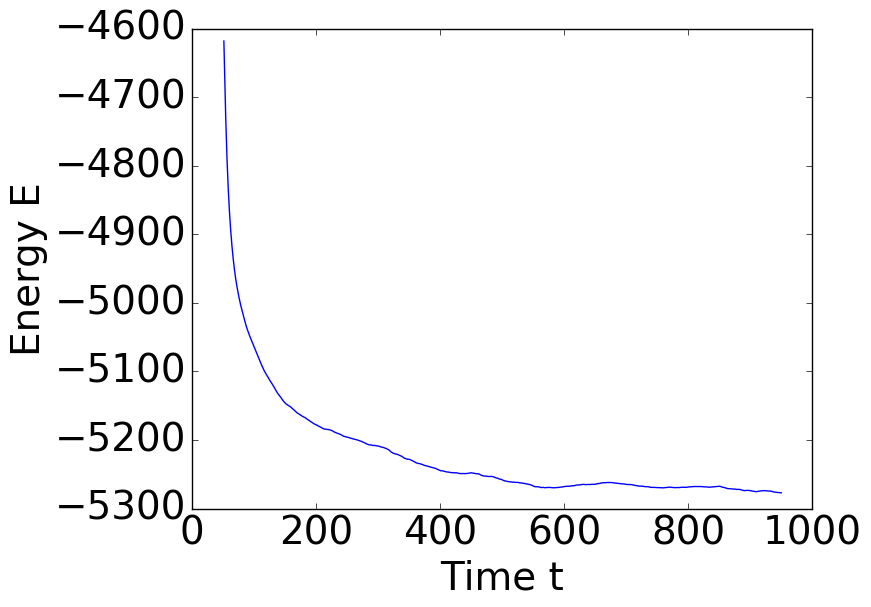
\includegraphics[width=\textwidth]{../dat/avTotal_Energy_T0d3_M100.png}
\end{subfigure}
\hfill
\begin{subfigure}{0.3\textwidth}
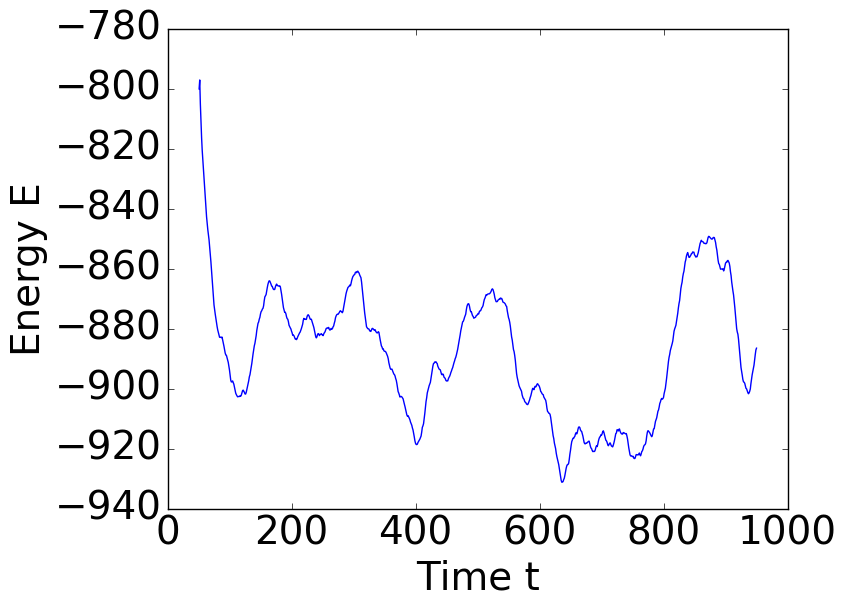
\includegraphics[width=\textwidth]{../dat/avTotal_Energy_T1d0_M100.png}
\end{subfigure}
\hfill
\begin{subfigure}{0.3\textwidth}
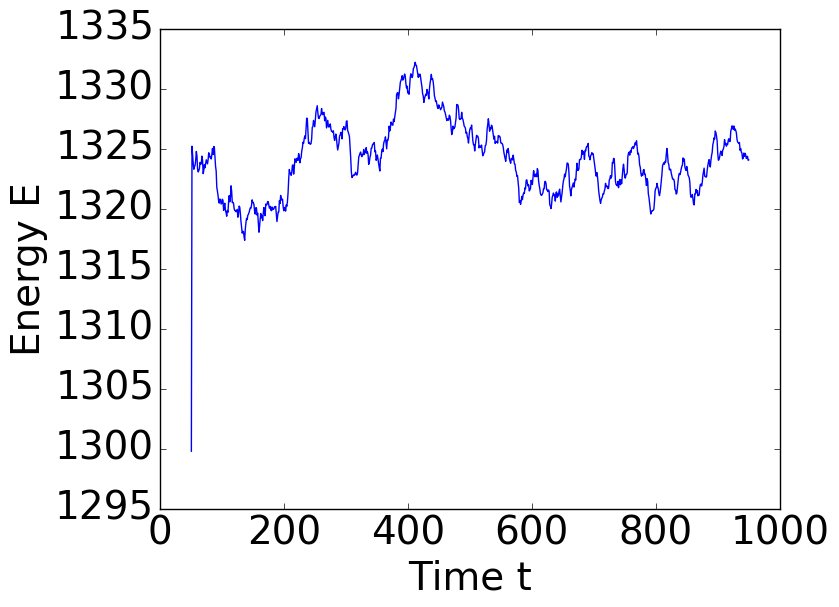
\includegraphics[width=\textwidth]{../dat/avTotal_Energy_T2d0_M100.png}
\end{subfigure}

P
\hfill
\begin{subfigure}{0.3\textwidth}
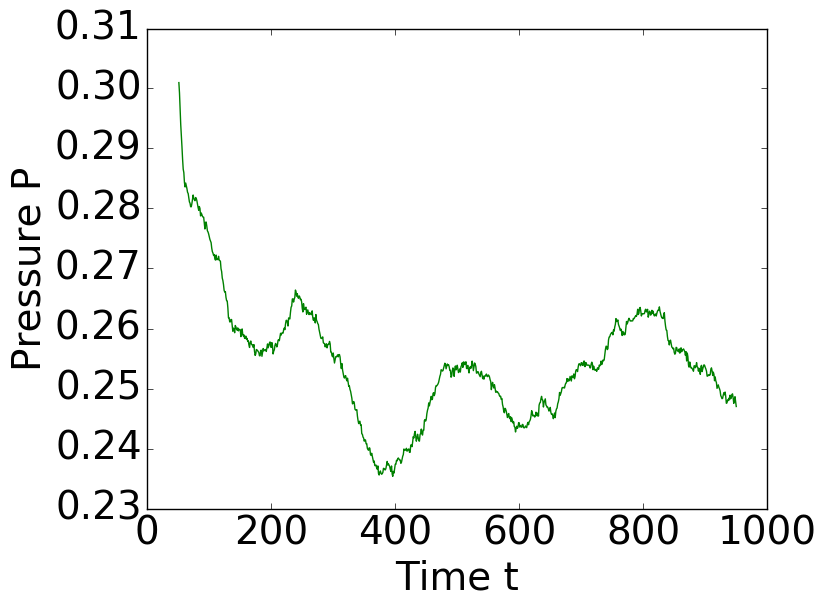
\includegraphics[width=\textwidth]{../dat/avPressure_T0d3_M100.png}
\end{subfigure}
\hfill
\begin{subfigure}{0.3\textwidth}
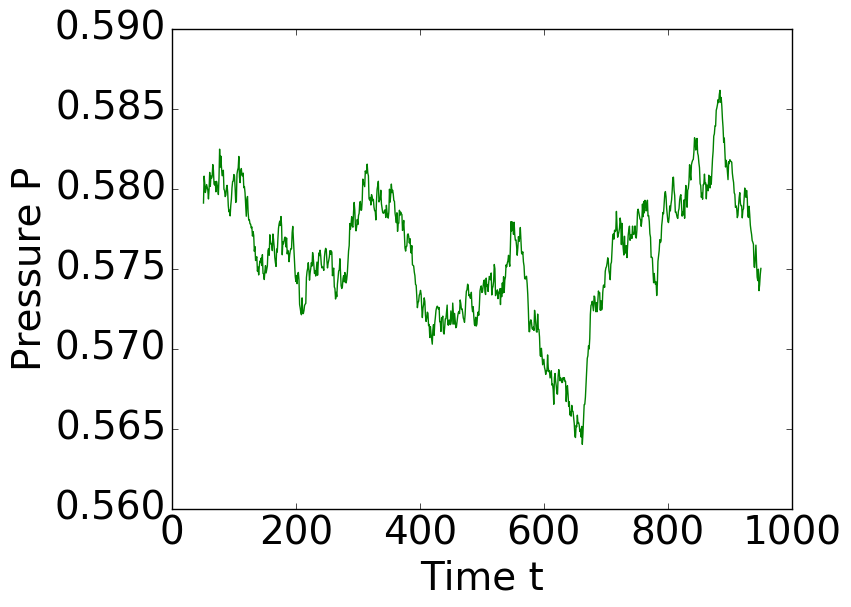
\includegraphics[width=\textwidth]{../dat/avPressure_T1d0_M100.png}
\end{subfigure}
\hfill
\begin{subfigure}{0.3\textwidth}
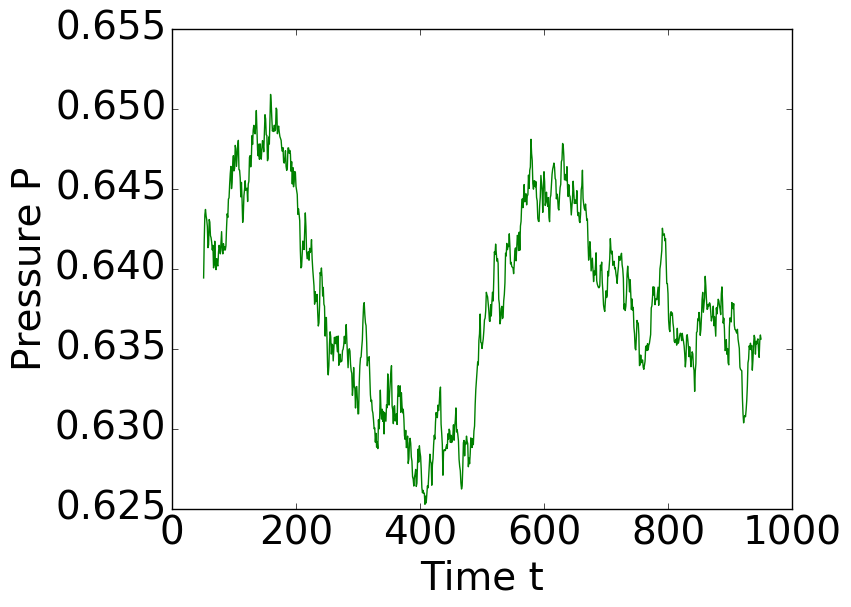
\includegraphics[width=\textwidth]{../dat/avPressure_T2d0_M100.png}
\end{subfigure}

\caption{
Measured Observables (Obs.) for a thermostat temperature $T_O$.\\
T is the real temperature of the system, E are the energies (green: potential, red: kinetic, blue: total).\\
U is the total energy of the system alone.\\
P is the pressure of the system.}
\label{fig4}
\end{figure}

\subsection*{Programming}

For the \emph{velocity rescaling} thermostat we can derive the rescaling-factor $\fr$ from equation \eqref{6fr1}.
\begin{align}
\frac{3}{2}k_BT_0
	&= \frac{\Ekino}{N}
	\label{6fr1}\\
&= \frac{1}{N}\sum_{i=1}^{N} \frac{(\fr\cdot\vecv{i})^2}{2m}
	\label{6fr2}\\
&= \fr^2\frac{\Ekin}{N}
	\label{6fr3}\\
&=\fr^2\frac{3}{2}k_BT
	\label{6fr4}\\
\fr
	&= \sqrt{\frac{T_0}{T}}
	\label{6r5}
\end{align}

This rescaling is implemented in C. In fact the implementation in C is not much faster than in python, but the thermostat in python did some crazy stuff.
The function c\_velocity\_rescaling can be seen in code block \ref{6rescaling}.

\listfile[MyCstyle]{../src/c_lj.cpp}{src/c\_lj.cpp}{281}{286}{Velocity rescaling}{6rescaling}

This function is used in the main loop in ljsim.py every time after meausuring the observalbles.\\

To start the thermostat you can use the command line option \ls{--tstat} which accepts the desired temperature as argument (see code block \ref{comsim}).
The option \ls{--ctstat} is there for continuing the simulation for the interrupted simulation with temperature T thermostat, but now with deactivated thermostat.
This is necessary because the programm saves the results of the simulation with different names for different temperatures.

\subsection*{Measurement}

Now we can test the simulation for desired temperatures of  $T\epsilon\left\lbrace 0.3,1.0,2.0\right\rbrace $. 
Therefor we must type into the command line:\\

\ls{>> python ljsim.py --tstat T0 --time 1000}.\\


Figure \ref{fig4} shows the results respectively.\\

We can easily see the system reach the desired temperature and the energies reach equilibrium. The pressure is a bit harder to see as the fluctuations are so large and take large amounts of time.\\

As you can see the equilibration time seems to be highest for $T_O=0.3$ and lowest for $T_O=2.0$. 
This is because the temperature $T_0=0.3$ is much lower than the initial temperature. 
Therefor the total energy of the system must decrease. But the positive kinetic energy is much lower, than the necessary energy differece. 
If the temperature should be $T=0.3$ the potential energy of the system must decrease, but it is not directly effected by the velocity rescaling.
By contrast for $T_0=2.0$ the necessary energy can simply  be reached by increasing the kinetic energy because it is much higher than the initial energy.
For $T_0=1.0$ the necessary energy is not much different from the initial one and therefor the other effects on equilibration have a higher influence.

\FloatBarrier
\section{Warming up the System}

When warming up the system you want to state a initial maximum force.
Therefor the command line option \ls{--warm} can be used (code block \ref{comsim}).
The option \ls{--cwarm} works analougus to \ls{--ctstat}.\\

The first thing needed is the function c\_force\_capping() which is implemented in C. 
The reason for this is because you have to do many if requests and calculations for each particle.

\listfile[MyCstyle]{../src/c_lj.cpp}{src/c\_lj.cpp}{288}{305}{Force capping}{7forcap}

The function in code block \ref{7forcap} limits the forces to a given maximum force fcap, but conserves the direction if the forces. 
Although this process is not physically correct.
Furthermore the function tests if no force is capped any more. 
When this is the case it sets fcap to zero.
The function is called in the vv\_step() function in ljsim.py.

\listfile{../src/ljsim.py}{src/ljsim.py}{164}{168}{Limiting forces}{7limfor}

As you can see, the function will not be activated any more if fcap = args.warm is set to zero.\\

At least the fcap should be increased by ten percent every time the measurements are done. 
This is done in code block \ref{7inc}.

\listfile{../src/ljsim.py}{src/ljsim.py}{213}{215}{Increase maximum force}{7inc}

But all the capping is useless without random initial conditions. 
The velocity is already random, so only the initial position has to be changed. 
You can do this with a similar command like in \ref{7rand}.

\listfile{../src/ljsim.py}{src/ljsim.py}{98}{101}{Random initial position}{7rand}





\end{document}
